\chapter{General details}

%%%%%%%%%%%%%%%%%%%%%%%%%%%%%%%%%%%%%%%%%%%%%%%%%%%%%%%%%%%%%%%%%%%%%%%%%%%%%%%%%%%%%%%%%%%%%%%%%%%%%%%%%%%%%
\section{Casas-Ibarra parametrization}
\label{sec:casas-ibarra}

It is known that when the structure of neutrino mass matrix has the form
%
\begin{align}
M^{\nu}=Y^{T}_{\nu}\Lambda Y_{\nu}  \,,
\end{align}
we are able to find the Yukawa couplings $Y_{\nu}$~\cite{Casas:2001sr,Ibarra:2003up}. 
In this section, we do a summary of how they are obtained.

First of all, we know that the PMNS matrix $U$ diagonalize the neutrino mass matrix, such that 
$U^T M^{\nu}U=\text{diag}(m_{\nu 1},m_{\nu 2},m_{\nu 3})=D_{m_\nu}$, and second, we will work in the basis in which the matrix $\Lambda$ is diagonal, such that, $\Lambda=D_{\Lambda}=\text{diag}(\Lambda_1,\Lambda_2,\Lambda_3)$. Therefore
%
\begin{align}
D_{m_\nu}=U^T M^{\nu}U=&U^TY_{\nu}^T\Lambda Y_{\nu}U = U^TY_{\nu}^TD_{\Lambda} Y_{\nu}U 
= U^TY_{\nu}^TD_{\sqrt{\Lambda}}D_{\sqrt{\Lambda}} Y_{\nu}U \,.
\end{align}
Multiplying by $D_{\sqrt{m_\nu^{-1}}}$ to both sides, we get
\begin{align}
D_{\sqrt{m_\nu^{-1}}}D_{\sqrt{m_\nu}}D_{\sqrt{m_\nu^{-1}}}= 1 =&
\left[D_{\sqrt{m_\nu^{-1}}}U^TY_{\nu}^TD_{\sqrt{\Lambda}}\right] \left[D_{\sqrt{\Lambda}} Y_{\nu}UD_{\sqrt{m_\nu^{-1}}}\right] \nonumber\\
=&\left[D_{\sqrt{\Lambda}} Y_{\nu} U D_{\sqrt{m_\nu^{-1}}}\right]^T \left[D_{\sqrt{\Lambda}} Y_{\nu}UD_{\sqrt{m_\nu^{-1}}}\right]\,.
\end{align}
In general, the last equation means that 
\begin{align}
\left[D_{\sqrt{\Lambda}} Y_{\nu}UD_{\sqrt{m_\nu^{-1}}}\right]=\mathcal{R}\,,
\end{align}
 is a $3\times 3$ complex orthogonal rotation matrix characterized by three angles (Euler-angles: $\theta_{12},\theta_{13},\theta_{23}$). Therefore, the Yukawa matrix $Y_{\nu}$ is given by
\begin{align}
Y_{\nu}=D_{\sqrt{\Lambda^{-1}}}\mathcal{R}D_{\sqrt{m_\nu}}U^{\dagger}\,,
\end{align} 
or 
\begin{align}
(Y_{\nu})_{ \alpha i}=&\frac{\sqrt{m_{\nu 1}}{\mathcal{R}}_{\alpha 1}U_{i1}^*+\sqrt{m_{\nu 2}}{\mathcal{R}}_{\alpha 2} U^{*}_{i2}+ \sqrt{m_{\nu 3}}{\mathcal{R}}_{\alpha 3} U^{*}_{i3}}{\sqrt{\Lambda_\alpha}}\,.
\end{align}

For the particular case of models with two particles circulating in the loop with associated $\Lambda_1$ and $\Lambda_2$ matrix elements (for instance, two scalar singlets in the SDFDM model), $\boldsymbol{\mathcal{R}}$ can be specified in terms of a single parameter~\cite{Casas:2001sr,Ibarra:2003up} as
\begin{align}
  \boldsymbol{\mathcal{R}}=&
  \begin{pmatrix}
    1 & \cos\theta & \sin\theta\\
    0 & -\sin\theta & \cos\theta\\
    0 &   0        & 1         \\ 
  \end{pmatrix} \,,
\end{align}
and therefore
\begin{align}
(Y_{\nu})_{1 i}=&\frac{\sqrt{m^\nu_2}\cos\theta U^{*}_{i2}+ \sqrt{m^\nu_3}\sin\theta U^{*}_{i3}}%
{\sqrt{\Lambda_1}}\,,\nonumber\\
(Y_{\nu})_{2 i}=&\frac{-\sqrt{m^\nu_2}\sin\theta U^{*}_{i2}+ \sqrt{m^\nu_3}\cos\theta U^{*}_{i3}}%
{\sqrt{\Lambda_2}}\,.
\end{align}












%%%%%%%%%%%%%%%%%%%%%%%%%%%%%%%%%%%%%%%%%%%%%%%%%%%%%%%%%%%%%%%%%%%%%%%%%%%%%%%%%%%%%%%%%%%%%%%%%%%%%%%%%%%%%%%%%
\section{Velocity averaged annihilation cross section $\langle \sigma v \rangle$ }
\label{sec:sigmav}
%
\begin{figure}[h]
\begin{center}
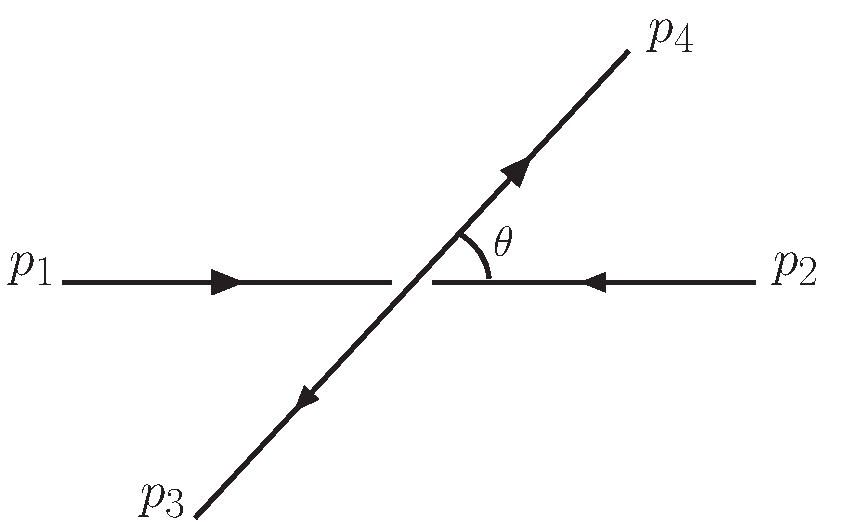
\includegraphics[scale=0.4]{CM}
\end{center}
\caption{Two particles scattering in the center of mass frame.}
\label{fig:cm-frame}
\end{figure}
%
It is known that for an scattering shown in Fig.~\ref{fig:cm-frame} the differential scattering cross section in the center of mass frame is given by
%
\begin{align}
\dfrac{d\sigma}{d\Omega}=&\dfrac{1}{64\pi^2s}\left[\dfrac{\left(s-(m_3+m_4)^2\right)\left(s-(m_3-m_4)^2\right)}{\left(s-(m_1+m_2)^2\right)\left(s-(m_1-m_2)^2\right)}\right]^{1/2}\overline{{|\mathcal{M}|^2}}\,.
\end{align}
%

The annihilation cross section $\sigma (s) $, for WIMPs of mass $m_1=m_2=m$ into to final states with masses $m_3$ and $m_4$ is given in terms of the dimensional factor $\Sigma$ which depend of the the variables $s$, $m$, $m_3$ and $m_4$ as~\cite{Chen:2013gya}
%
\begin{align}
\label{eq:cs-2to2}
\sigma(s)=\dfrac{1}{32\pi m^2}\sqrt{\dfrac{4m^2}{s}}\sqrt{\dfrac{m^2}{s-4m^2}}\sqrt{1-\dfrac{(m_3+m_4)^2}{s}}\sqrt{1-\dfrac{(m_3-m_4)^2}{s}}\,
\Sigma(s;m,m_2,m_3)\,.
\end{align} 
%
where $\Sigma(s;m,m_2,m_3)$ is given in terms of the matrix element $\mathcal{M}$ by
%
\begin{align}
\Sigma(s;m,m_2,m_3)
= & \int \dfrac{d\Omega}{4\pi}\dfrac{1}{4}\sum_{s_3s_4}\sum_{r_3,r_4}|\mathcal{M}|^2
=   \int \dfrac{d\Omega}{4\pi}\overline{|\mathcal{M}|^2}  \hspace{1.0 cm} \text{fermionic WIMPs}\\
= & \int \dfrac{d\Omega}{4\pi}\sum_{r_3,r_4}|\mathcal{M}|^2 
=   \int \dfrac{d\Omega}{4\pi}\overline{|\mathcal{M}|^2} \hspace{2.0 cm} \text{bosonic WIMPs}\,,
\end{align}
%
where initial spins states $s_3 , s_4$ are averaged over the fermionic WIMPs, and polarization $r_3 , r_4$ of the final states bosons are summed over. The integral in the solid angles has an extra factor of $1/2$ if the two final state particles are identical, for example $\chi\chi\to\gamma\gamma$.  
%
We will use this expression in order to compute the velocity averaged annihilation cross section $\langle \sigma v \rangle$ for the DM annihilation into $\gamma\gamma$ and $\gamma Z$. 

%%%%%%%%%%%%%%%%%%%%%%%%%%%%%%%%%%%%%%%%%%%%%%%%%%%
\subsubsection{$\langle\sigma v_r\rangle$ for DM annihilation into $\gamma\gamma$}
For the case of DM annihilation into two photons, $\chi^0\chi^0\rightarrow\gamma\gamma$: $m_1=m_2=m$, $m_3=m_4=0$, $s=(p_1+p_2)^2=p_1^2+p_2^2+2p_1\cdot p_2=4m^2(1+(v_r/2)^2)$ with $v_r$ the relative velocity of the DM particles in the initial state.
The scattering cross section~\eqref{eq:cs-2to2} is
%
\begin{align}
\langle\sigma v_r\rangle=&\dfrac{1}{32\pi m^2}\overline{{|\mathcal{M}|^2}}\left(1-\dfrac{v_r^2}{8}+\mathcal{O}(v_r^4)\right)\,,
\end{align}
%
where we show the s-wave and p-wave contribution explicitly. In the limit of zero velocity we have the s-wave contribution
%
\begin{align}
\langle\sigma v_r\rangle|_{\text{s-wave}}=\dfrac{1}{32\pi m^2}\overline{{|\mathcal{M}|^2}}\,.
\end{align}
%
\noindent
{\color{red}NOTA}: The natural units of $\langle\sigma v_r\rangle$ are $E^{-2}$. In order to change to international unit system (MKS) we use next the relations:
\begin{align*}
10^{-13} \text{cm} = & 1 \text{fermi (fm)}=5.068\text{ GeV}^{-1} \to
10^{-27} \text{cm}^2 = 2.56 \text{ GeV}^{-2} \\
1 \text{ sec} =& 3\times10^{10} \text{cm} \\
\slashed{h}c =& 197.3 \text{ MeV }\text{fm}=197.3\times10^{-3} \text{GeV} 10^{-13} \text{cm}=197.3\times10^{-16} \text{GeV cm}\,,
\end{align*}
%
therefore, if we wan to to change the units of the $\langle\sigma v_r\rangle$, we need to multiply for the factor:
$(197.3\times 10^{-16} \text{GeV cm})^2 (3\times 10^8\times 10^2 \text{cm/sec})$.










%%%%%%%%%%%%%%%%%%%%%%%%%%%%%%%%%%%%%%%%%%%%%%%%%%%%%%%%%%%%%%%%%%%%%%%%%%%%%%%%%%%%%%%%%%%%%%%%%%%%%%%%%%%%%%
\section{Passarino-Veltman One-loop integrals}
\label{sec:passarino-veltman}

\begin{figure}[h]
\centering
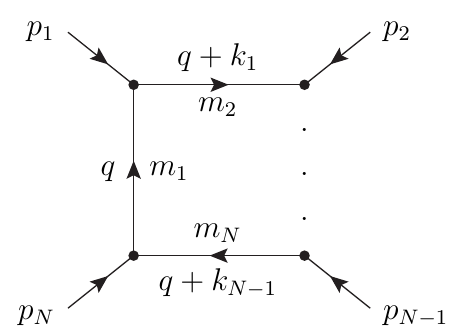
\includegraphics[scale=0.55]{n-points-diagram2}
\caption{General One-loop diagram. \textsc{LoopTools}'s convention~\cite{Hahn:1998yk}.}
\end{figure}

The n-point tensor integral in the \textsc{LoopTools}'s convention~\cite{Hahn:1998yk} is given by:
\begin{align}
\label{eq:n-point-integral}
T^N_{\mu_{1}\cdots\mu_{P}}(k_i)=&\dfrac{\mu^{4-D}}{i\pi^{D/2}r_{\Gamma}}\int d^Dq \dfrac{q_{\mu_1}\cdots q_{\mu_P}}{[q^2-m_1^2][(q+k_1)^2-m_2^2]\cdots[(q+k_{N-1})^2-m_{N}^2]}\,,
\end{align} 
with
\begin{align}
r_{\Gamma}=\dfrac{\Gamma^2(1-\epsilon)\Gamma(1+\epsilon)}{\Gamma(1-2\epsilon)}\hspace{1.0 cm} D=4-2\epsilon \,.
\end{align} 
\label{eq:ptok}
The momenta $k_i$ that appear in the denominators are related to the external momenta $p_i$ as
\begin{align}
p_1=& k_1 \hspace{1 cm} p_2=k_2-k_1 \hspace{1 cm} \cdots \hspace{1 cm} p_N=k_N-k_{N-1}\nonumber \\
k_1=& p_1 \hspace{1 cm} k_2=p_1+p_2 \hspace{1 cm} \cdots \hspace{1 cm} k_N=\sum_{i=1}^N p_i\,.
\end{align}
%
In general, the \textsc{LoopTools} notation for the n-point integrals is: $A=T^1$, $B=T^2$, $C=T^3$ and $D=T^4$. Therefore, regarding to the Eq.~\eqref{eq:n-point-integral} we have that
%
\begin{align}
\label{eq:A-point-integral}
A_0;A_{\mu}\left(m^2 \right)=&\dfrac{\mu^{4-D}}{i\pi^{D/2}r_{\Gamma}}\int d^Dq \dfrac{ 1;q_{\mu} }{[q^2-m^2]} \,,
\end{align} 
%
\begin{align}
\label{eq:B-point-integral}
B_0;B_{\mu};B_{\mu\nu}\left(p_1^2,m_1^2,m_2^2 \right) 
=&\dfrac{\mu^{4-D}}{i\pi^{D/2}r_{\Gamma}}\int d^Dq \dfrac{ 1;q_{\mu};q_{\mu}q_{\nu} }{[q^2-m_1^2][(q+k_1)^2-m_2^2]} \,,
\end{align} 
%
\begin{align}
\label{eq:C-point-integral}
C_0;C_{\mu};C_{\mu\nu};C_{\mu\nu\rho}&\left(p_1^2,p_2^2,(p_1+p_2)^2,m_1^2,m_2^2,m_3^2\right) \nonumber\\
=&\dfrac{\mu^{4-D}}{i\pi^{D/2}r_{\Gamma}}\int d^Dq \dfrac{ 1;q_{\mu};q_{\mu}q_{\nu};q_{\mu}q_{\nu}q_{\rho} }{[q^2-m_1^2][(q+k_1)^2-m_2^2][(q+k_2)^2-m_3^2]} \,,
\end{align} 
%
\begin{align}
\label{eq:D-point-integral}
D_0;D_{\mu};D_{\mu\nu};D_{\mu\nu\rho};D_{\mu\nu\rho\sigma}&\left(p_1^2,p_2^2,p_3^2,p_4^2,(p_1+p_2)^2,(p_2+p_3)^2,m_1^2,m_2^2,m_3^2,m_4^2\right) \nonumber\\
=&\dfrac{\mu^{4-D}}{i\pi^{D/2}r_{\Gamma}}\int d^Dq \dfrac{ 1;q_{\mu};q_{\mu}q_{\nu};q_{\mu}q_{\nu}q_{\rho};q_{\mu}q_{\nu}q_{\rho}q_{\sigma} }{[q^2-m_1^2][(q+k_1)^2-m_2^2][(q+k_2)^2-m_3^2][(q+k_3)^2-m_4^2]} \,,
\end{align} 
%
which are shown in Fig.~\ref{fig:n-point-diagrams}.
%
\begin{figure}[h]
\centering
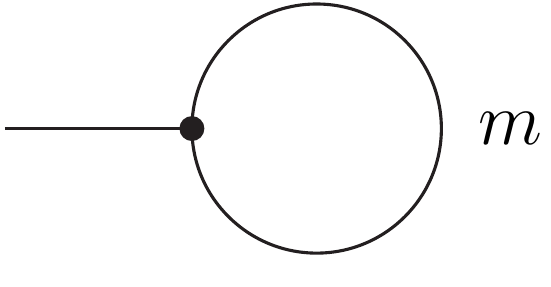
\includegraphics[scale=0.24]{1-points-diagram} \hspace{1 cm}
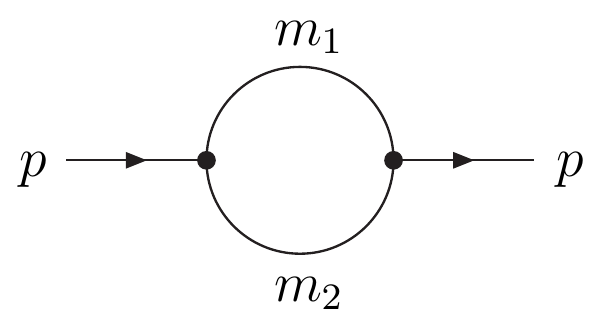
\includegraphics[scale=0.32]{2-points-diagram} 

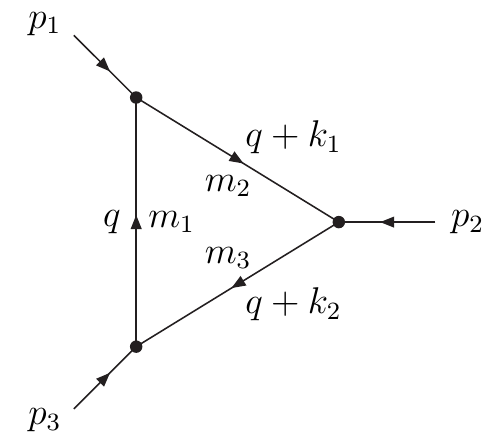
\includegraphics[scale=0.37]{3-points-diagram}\hspace{1 cm}
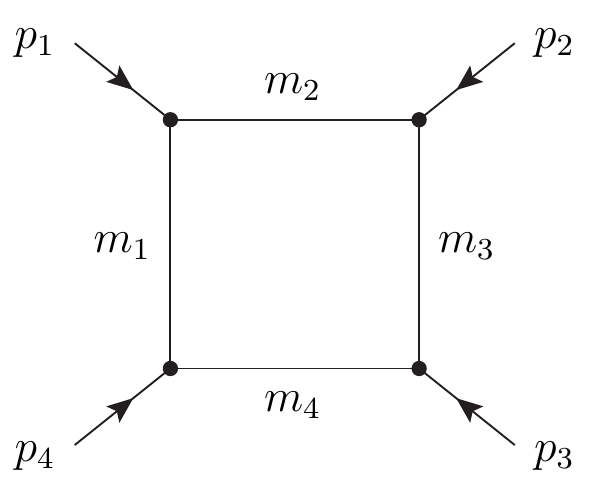
\includegraphics[scale=0.27]{4-points-diagram}
\caption{$A$, $B$, $C$ and $D$ point functions.}
\label{fig:n-point-diagrams}
\end{figure}


\subsection{Tensor Coefficients}
\label{sec:tensor-coefficients}

$\index{tensor coefficients}%
$\index{Lorentz-covariant tensors}%
The integrals with a tensor structure can be reduced to integrals multiplied by linear
combinations of Lorentz-covariant tensors constructed from the metric
tensor $g_{\mu\nu}$ and a linearly independent set of the momenta~\cite{Passarino:1978jh}~\footnote{The choice of this basis is not unique. 
For example, \textsc{LoopTools} chooses the basis of the $k_i$ momenta instead the external momenta $p_i$.
}.
%
\textsc{LoopTools} provides not the tensor integrals themselves, but the coefficients of
these Lorentz-covariant tensors.  It works in a basis formed from
$g_{\mu\nu}$ and the momenta $k_i$, which are the sums of the external
momenta $p_i$ (see Eq.~\eqref{eq:ptok})~\cite{Denner:1991kt}, with the advantage that in this basis
the tensor-coefficient functions are totally symmetric in their indices.

For the integrals up to the four-point function the decomposition reads
explicitly as
\begin{align*}
B_\mu &=
	k_{1\mu} B_1\,,
	\displaybreak[0] \\
B_{\mu\nu} &=
	g_{\mu\nu} B_{00} + k_{1\mu} k_{1\nu} B_{11}\,,
	\displaybreak[0] \\[1ex]
C_\mu &=
	k_{1\mu} C_1 + k_{2\mu} C_2 = \sum_{i=1}^2 k_{i\mu} C_i\,,
	\displaybreak[0] \\
C_{\mu\nu} &=
	g_{\mu\nu} C_{00} + \sum_{i,j=1}^2 k_{i\mu} k_{j\nu} C_{ij}\,,
	\displaybreak[0] \\
C_{\mu\nu\rho} &=
	\sum_{i=1}^2 \bigl(
	g_{\mu\nu} k_{i\rho}
	+ g_{\nu\rho} k_{i\mu}
	+ g_{\mu\rho} k_{i\nu}\bigr) C_{00i}+
	\sum_{i,j,\ell=1}^2 k_{i\mu} k_{j\nu} k_{\ell\rho} C_{ij\ell}\,,
	\displaybreak[0] \\[1ex]
D_\mu &=
	\sum_{i=1}^3 k_{i\mu} D_i\,,
	\displaybreak[0] \\
D_{\mu\nu} &=
	g_{\mu\nu} D_{00} + \sum_{i,j=1}^3 k_{i\mu} k_{j\nu} D_{ij}\,,
	\displaybreak[0] \\
D_{\mu\nu\rho} &=
	\sum_{i=1}^3\bigl(
	g_{\mu\nu} k_{i\rho}
	+ g_{\nu\rho} k_{i\mu}
	+ g_{\mu\rho} k_{i\nu}\bigr) D_{00i}
	+ \sum_{i,j,\ell=1}^3 k_{i\mu} k_{j\nu} k_{\ell\rho} D_{ij\ell}\,,
	\displaybreak[0] \\
D_{\mu\nu\rho\sigma} &=
	(g_{\mu\nu} g_{\rho\sigma}
	+ g_{\mu\rho} g_{\nu\sigma}
	+ g_{\mu\sigma} g_{\nu\rho}) D_{0000} \\
	& \hphantom{=} + \sum_{i,j=1}^3 \bigl(
	g_{\mu\nu} k_{i\rho} k_{j\sigma}
	+ g_{\nu\rho} k_{i\mu} k_{j\sigma}
	+ g_{\mu\rho} k_{i\nu} k_{j\sigma} \\[-1.5ex]
	& \hphantom{=+\sum_{i,j=1}^3\bigl(\,}
	+ g_{\mu\sigma} k_{i\nu} k_{j\rho}
	+ g_{\nu\sigma} k_{i\mu} k_{j\rho}
	+ g_{\rho\sigma} k_{i\mu} k_{j\nu}\bigr) D_{00ij} \\[-1ex]
	& \hphantom{=} + \sum_{i,j,\ell,m=1}^3
	k_{i\mu} k_{j\nu} k_{\ell\rho} k_{m\sigma} D_{ij\ell m}\,.
\end{align*}
Of all scalar and tensor-coefficient functions, only 
$A_0$, $B_0$, $B_1$, $B_{00}$, $B_{11}$, $B_{001}$, $B_{111}$, $B'_{00}$,
the C coefficients with at least two indices zero, and the D coefficients
with at least four indices zero are actually UV divergent~\cite{Hahn:1998yk}.


\subsection{Conventions for the Momenta}

%\index{momenta!conventions for}%
A large source of mistakes is the way of specifying the momentums in the
one-loop integrals.  The prime error in this respect is the confusion of
the external momenta $p_i$ with the momenta $k_i$ appearing in the
denominators, which are the sums of the $p_i$ (see Eq.~\eqref{eq:ptok}).
%
It is important to realize that \textsc{LoopTools} functions like $C_1$ and
$C_{112}$ are the coefficients respectively of $k_{1\mu}$ and $k_{1\mu}
k_{1\nu} k_{2\rho}$, not of $p_{1\mu}$ and $p_{1\mu} p_{1\nu} p_{2\rho}$.









%%%%%%%%%%%%%%%%%%%%%%%%%%%%%%%%%%%%%%%%%%%%%%%%%%%%%%%%%%%%%%%%%%%%%%%%%%%%%%%%%%%%%%%%%%%%%%%%%%%%%
\subsection{$C$ and $D$ reduction to scalar integrals}
\label{sec:CD-reduction}

The original Passarino-Veltman squema~\cite{Passarino:1978jh} is based in the assumption of independent external momenta $p_i$. When the momenta are linearly dependent the Gram Determinant of the momenta goes to zero and the Passarino-Veltmann scheme breaks down. In that case, we can deal with this problem reducing the n-point integrals to a linear combination of $(n-1)$-point integrals as we will describe.
  
In general, the n-point scalar integral is:
\begin{align}
\label{eq:n-point-scalar}
T^N_0(k_i)=&\dfrac{\mu^{4-D}}{i\pi^{D/2}r_{\Gamma}}\int d^Dq \dfrac{1}{[q^2-m_1^2][(q+k_1)^2-m_2^2]\cdots[(q+k_{N-1})^2-m_{N}^2]}\nonumber\\
=&\dfrac{\mu^{4-D}}{i\pi^{D/2}r_{\Gamma}}\int d^Dq \dfrac{1}{N_1N_2\cdots N_N}\,,
\end{align} 
with
\begin{align}
N_i=& (q+k_{i-1})^2-m_i^2 \,, \hspace{1 cm} i=1,\cdots N \hspace{1 cm} k_0=0\,.
\end{align}
In the case of degeneration in the momenta, $T^N_0(k_i)$ can be expanded by $T^{N-1}_0(k_i)$ in the next form:
%
\begin{align}
\label{eq:int-reduction}
T_0^N=\sum_{i=1}^{N}\alpha_i\left(\dfrac{\mu^{4-D}}{i\pi^{D/2}r_{\Gamma}}\int d^Dq \dfrac{1}{N_1N_2\cdots N_{i-1}N_{i+1}\cdots N_N}\right)
=\sum_{i=1}^{N}\alpha_i\,T_0^{N-1}(i)\,.
\end{align}
In order to know the necessary condition to find the $\alpha_i$ coefficients we can use the Eq.~\eqref{eq:n-point-scalar} and \eqref{eq:int-reduction}. In means that we  have to fulfill
\begin{align}
\dfrac{1}{N_1N_2\cdots N_N}= \dfrac{\alpha_1}{N_2N_3\cdots N_N}+\dfrac{\alpha_2}{N_1N_3\cdots N_N}+\cdots +\dfrac{\alpha_N}{N_1N_2N_3\cdots N_{N-1}}
=\dfrac{\sum_{i=1}^N\alpha_iN_i}{N_0N_1\cdots N_N}\,,
\end{align}
%
therefore
%
\begin{align}
1=\sum_{i=1}^N\alpha_iN_i=\sum_{i=1}^N\alpha_i(q^2+2q_{\mu}k_{i-1}^{\mu}+k_{i-1}^2-m_{i}^2)
=q^2\sum_{i=1}^N\alpha_i + 2q_{\mu}\sum_{i=1}^N\alpha_ik_{i-1}^{\mu} + \sum_{i=1}^N\alpha_i (k_{i-1}^2-m_i^2)\,.
\end{align}
%
Now, in order to satisfy this condition for all momenta $q_{\mu}$, we have to guarantee the next three relations:
\begin{align}
\sum_{i=1}^N\alpha_i = 0 \hspace{1 cm}
\sum_{i=1}^N\alpha_ik_{i-1} = 0  \hspace{1 cm}
\sum_{i=1}^N\alpha_i (k_{i-1}^2-m_i^2) =& 1\,.
\end{align}
In particular, the second condition guaranteed that
\begin{align}
\alpha_2k_1+\alpha_3k_2+\alpha_4k_3\cdots \alpha_{N}k_{N-1}=0\,.
\end{align}
%
If the set of momenta $\{k_1, k_2 \cdots k_{N-1}\}$ are $(N-1)$ linear independent, we will have the  trivial solution $\alpha_i=0$ for all $i$. Now, in order to don't have the trivial solution, the $k_i$ momenta must be linearly dependent as the preliminary condition when the Passarino-Veltman scheme breaks down.

The last scheme is general for reduce an $n$-point integral to a $(n-1)$-point integral. We will focus in the particular case of $N=3$ and $N=4$.
%
For $N=3$, the $C$ scalar integral can be reduced to $B$ $(N=2)$ if you satisfied the next three relations
\begin{align}
\sum_{i=1}^N\alpha_i = 0 \hspace{0.5 cm} &\rightarrow \hspace{0.5  cm} \alpha_1+\alpha_2+\alpha_3=0 \\
\sum_{i=1}^N\alpha_ik_{i-1} = 0 \hspace{0.5  cm} &\rightarrow \hspace{0.5  cm} \alpha_2k_1+\alpha_3k_2=\alpha_2p_1+\alpha_3(p_1+p_2)=0 \nonumber \\ 
& \Rightarrow \hspace{0.5  cm} \alpha_2p_1^2+\alpha_3(p_1^2+p_1\cdot p_2)= \alpha_2p_1^2+\alpha_3\dfrac{(p_1^2-p_2^2+p_3^2)}{2}=0 \\
\sum_{i=1}^N\alpha_i (k_{i-1}^2-m_i^2) = 1\hspace{0.5  cm} &\rightarrow \hspace{0.5  cm} 
-\alpha_1m_1^2+ \alpha_2(k_1^2-m_2^2)+ \alpha_3(k_2^2-m_3^2)\nonumber\\
&\hspace{0.6 cm}=-\alpha_1m_1^2+ \alpha_2(p_1^2-m_2^2)+ \alpha_3(p_3^2-m_3^2)=1\,,
\end{align} 
which are summary in the next system of equation:
\begin{align}
\begin{pmatrix}
1 & 1 & 1 \\
0 & p_1^2 & (p_1^2-p_2^2+p_3^2)/2 \\
 -m_1^2 & (p_1^2-m_2^2) & (p_3^2-m_3^2)
\end{pmatrix}
\begin{pmatrix}
\alpha_1 \\ \alpha_2 \\ \alpha_3
\end{pmatrix}=
\begin{pmatrix}
0 \\ 0 \\ 1
\end{pmatrix}\,.
\end{align}
%
Explicitly, according to the Eq.~\eqref{eq:int-reduction}
\begin{align}
\label{eq:t30}
T^3_0=& \left(\dfrac{\mu^{4-D}}{i\pi^{D/2}r_{\Gamma}}\int d^Dq \dfrac{\alpha_1}{N_2N_3}\right)
+\left(\dfrac{\mu^{4-D}}{i\pi^{D/2}r_{\Gamma}}\int d^Dq \dfrac{\alpha_2}{N_1N_3}\right)
+\left(\dfrac{\mu^{4-D}}{i\pi^{D/2}r_{\Gamma}}\int d^Dq \dfrac{\alpha_3}{N_1N_2}\right)\,,
\end{align}
or equivalent:
\begin{align}
C_0(1,2,3)=&\alpha_3B_0(1,2)+\alpha_2B_0(1,3) +\alpha_1B_0(2,3)\nonumber \\
=& \alpha_{12}B_0(1,2)+\alpha_{13}B_0(1,3)+\alpha_{23}B_0(2,3)\,, 
\end{align}
where $C(i,j,k)$ means the three-point functions with denominator $N_iN_jN_k$. The same for $B(i,j)$. 
Notice that we change the notation for the coefficients $\alpha_i$ in order to get a more compact notation. 

Analogously, for $N=4$, the $D$ scalar integrals can be reduced to $C$ $(N=3)$ scalar integrals and the coefficient can be found solving the next matrix equation
\begin{align}
\begin{pmatrix}
1 & 1 & 1 & 1 \\
0 & p_1^2 & (p_1^2-p_2^2+p_5^2)/2  & (p_1^2+p_4^2-p_6^2)/2\\
0 & (-p_1^2-p_2^2+p_5^2)/2 & (-p_1^2+p_2^2+p_5^2)/2  & (-p_1^2-p_3^3+p_5^2+p_6^2)/2\\
 -m_1^2 & p_1^2-m_2^2 & p_5^2-m_3^2 & p_4^2-m_4^2
\end{pmatrix}
\begin{pmatrix}
\alpha_{234} \\ \alpha_{134} \\ \alpha_{124} \\ \alpha_{123}
\end{pmatrix}=
\begin{pmatrix}
0 \\ 0 \\ 0 \\ 1
\end{pmatrix}\,,
\end{align}
%
with $p_5=p_1+p_2$ and $p_6=p_2+p_3$.
%
The scalar reduction in this case is
\begin{align}
D_0(1,2,3,4)= \alpha_{123}C_0(1,2,3)+\alpha_{124}C_0(1,2,4)+\alpha_{134}C_0(1,3,4)+\alpha_{234}C_0(2,3,4)\,.
\end{align}

For the case of tensor reduction we have to take care that \textsc{LoopTools} works in the base of the $k_i$ momenta as we described in the Sec.~\ref{sec:tensor-coefficients}. 
%
We are interested only in the reduction of the four-point integrals $D_{\mu}$, $D_{\mu\nu}$,$D_{\mu\nu\rho}$ to three-point functions, because in general the three, two and one-point functions have analytically representation that we are able to find. 

For $D_{\mu}$ tensor we have
%
\begin{align}
\label{eq:du}
D_{\mu} = &\int d^Dq \dfrac{ q_{\mu} }{[q^2-m_1^2][(q+k_1)^2-m_2^2][(q+k_2)^2-m_3^2][(q+k_3)^2-m_4^2]}
=\int d^Dq \dfrac{ q_{\mu} }{[1][2][3][4]} \nonumber \\
=&\alpha_{123}\int d^Dq \dfrac{ q_{\mu} }{[1][2][3]} 
+\alpha_{124}\int d^Dq \dfrac{ q_{\mu} }{[1][2][4]} 
+\alpha_{134}\int d^Dq \dfrac{ q_{\mu} }{[1][3][4]} 
+\alpha_{234}\int d^Dq \dfrac{ q_{\mu} }{[2][3][4]}\,. 
\end{align} 
%
We omit the factor $\dfrac{\mu^{4-D}}{i\pi^{D/2}r_{\Gamma}}$ in the last equation in order to have a more compact notation. To continue, we have to take some care with the last integral. It does not have the canonical definition of the three point functions because the first propagator has an external momenta $k_1=p_1$. In order to have the canonical definition, we can do a simple change of variable $q+k_1\rightarrow q^{'}$ 
\begin{align}
\label{eq:c234}
\int d^Dq \dfrac{ q_{\mu} }{[2][3][4]}=&\int d^Dq \dfrac{ q_{\mu} }{[(q+k_1)^2-m_2^2][(q+k_2)^2-m_3^2][(q+k_3)^2-m_4^2]}\nonumber \\
=& \int d^Dq \dfrac{ (q_{\mu}-k_{1\mu}) }{[q^2-m_2^2][(q+(k_2-k_1))^2-m_3^2][(q+(k_3-k_1))^2-m_4^2]}\nonumber \\
=& \tilde{C}_{\mu}(2,3,4)-k_{1\mu}\tilde{C}_0(2,3,4)\,,
\end{align}
where the tilde means that we have to take care of the last shift in the propagator's momenta.

Replacing the Eq.~\eqref{eq:c234} in the Eq.~\eqref{eq:du} and using the definition of the $C_{\mu}$ tensor, we have
%
\begin{align}
D_{\mu}=& \alpha_{123}C_{\mu}(1,2,3)+\alpha_{124}C_{\mu}(1,2,4)+\alpha_{134}C_{\mu}(1,3,4) +\alpha_{234}\left(\tilde{C}_{\mu}(2,3,4)-k_{1\mu}\tilde{C}_0(2,3,4)\right)\,.
\end{align} 

Finally, using the definition of the tensor coefficients given in the Sec.~\ref{sec:tensor-coefficients} we have that
%
\begin{align}
D_{\mu}=&\alpha_{123}\left(k_{1\mu}C_1(1,2,3)+k_{2\mu}C_2(1,2,3)\right)
+\alpha_{124}\left(k_{1\mu}C_1(1,2,4)+k_{3\mu}C_2(1,2,4)\right)\nonumber \\
+&\alpha_{134}\left(k_{2\mu}C_1(1,3,4)+k_{3\mu}C_2(1,3,4)\right)\nonumber \\
+&\alpha_{234}\left((k_{2\mu}-k_{1\mu})\tilde{C}_1(2,3,4)+(k_{3\mu}-k_{1\mu})\tilde{C}_2(2,3,4)-k_{1\mu}\tilde{C}_0(2,3,4)\right)\,.
\end{align}
%
But for definition $D_{\mu}=k_{1\mu}D_1+k_{2\mu}D_2+k_{3\mu}D_3$, therefore, doing the matching in the momenta $k_i$, we have the relation between the coefficients tensor of $D$ and $C$ functions
\begin{align}
\label{eq:Di-reduction}
D_0=& \alpha_{123}C_0+\alpha_{124}C_0+\alpha_{134}C_0+\alpha_{234}\tilde{C}_0\nonumber \\
D_1=&\alpha_{123}C_1+\alpha_{124}C_1+0*\alpha_{134}C_1-\alpha_{234}\left(\tilde{C}_0+\tilde{C}_1+\tilde{C}_2\right)\nonumber \\
D_2=&\alpha_{123}C_2+0*\alpha_{124}C_1+\alpha_{134}C_1+\alpha_{234}\tilde{C}_1\nonumber \\
D_3=&0*\alpha_{123}C_1+\alpha_{124}C_2+\alpha_{134}C_2+\alpha_{234}\tilde{C}_2\,,
\end{align}
where we included the scalar reduction for $D_0$ found before and a more compact notation $\alpha_{ijk}C_l=\alpha_{ijk}C_l(ijk)$.

Analogically, for $D_{\mu\nu}$ tensor reduction we found

\begin{align}
\label{eq:Dij-reduction}
D_{00}=& \alpha_{123}C_{00}+\alpha_{124}C_{00}+\alpha_{134}C_{00}+\alpha_{234}\tilde{C}_{00}\nonumber \\
D_{11}=&\alpha_{123}C_{11}+\alpha_{124}C_{11}+0*\alpha_{134}C_1+\alpha_{234}\left(\tilde{C}_0+2\tilde{C}_1+2\tilde{C}_2+\tilde{C}_{11}+2\tilde{C}_{12}+\tilde{C}_{22}\right)\nonumber \\
D_{12}=&\alpha_{123}C_{12}+0*\alpha_{124}C_{22}+0*\alpha_{134}C_{22}-\alpha_{234}\left(\tilde{C}_{1}+\tilde{C}_{11}+\tilde{C}_{12}\right)\nonumber\\
D_{13}=&0*\alpha_{123}C_{12}+\alpha_{124}C_{12}+0*\alpha_{134}C_{22}-\alpha_{234}\left(\tilde{C}_{12}+\tilde{C}_{2}+\tilde{C}_{22}\right)\nonumber\\
D_{22}=&\alpha_{123}C_{22}+0*\alpha_{124}C_1+\alpha_{134}C_{11}+\alpha_{234}\tilde{C}_{11}\nonumber \\
D_{23}=&0*\alpha_{123}C_{22}+0*\alpha_{124}C_1+\alpha_{134}C_{12}+\alpha_{234}\tilde{C}_{12}\nonumber \\
D_{33}=&0*\alpha_{123}C_{22}+\alpha_{124}C_{22}+\alpha_{134}C_{22}+\alpha_{234}\tilde{C}_{22}\,,
\end{align}

and for $D_{00i}$ tensor reduction we found

\begin{align}
\label{eq:D00i-reduction}
D_{001} =& \alpha_{123}C_{001}+\alpha_{124}C_{001}+0*\alpha_{134}C_{00}-\alpha_{234}\left(\tilde{C}_{00}+\tilde{C}_{001}+\tilde{C}_{002}\right)\nonumber \\
D_{002} =& \alpha_{123}C_{002}+0*\alpha_{124}C_{001}+\alpha_{134}C_{001}+\alpha_{234}\tilde{C}_{001}\nonumber \\
D_{003} =& 0*\alpha_{123}C_{00}+\alpha_{124}C_{002}+\alpha_{134}C_{002}+\alpha_{234}\tilde{C}_{002}\,.
\end{align}

\noindent
For another and complete reduction of the tensor n-point $T^N_{\mu_1\cdots \mu_{P}}$ integrals but in another base, see the Ref.~\cite{STUART1988367}. For us, that scheme is not useful because we are working in the base of the momenta $k_i$, that is not the base used in that work. 









%%%%%%%%%%%%%%%%%%%%%%%%%%%% Non Linear Gauge  %%%%%%%%%%%%%%%%%%%%%%%%%%%%%%%%%

\section{Non-linear $R_\xi$ gauges}
\label{sec:Gauge}
\subsection{Charged gauge bosons }

\begin{comment}
The most general Lagrangian for a charged gauge boson $\phi_\mu$ is 

\begin{equation}
%
{\cal L }\bigg|_{\substack{\text{Vector}\\\text{Mediators}}} =-\frac{1}{2}\left({\cal D}_\mu \medpVcov{\nu} -{\cal D}_\nu \medpVcov{\mu} \right)\left({\cal D}^\mu \medp^{\nu} -{\cal D}^\nu \medp^{\mu} \right)+ \mmed^2\, \medm^{\mu}\medp_\mu+ie\,{\cal abcdefghijklmnopqrstuvwxyz}F^{\mu\nu} \medp_\mu\medpVcov{\nu} +\delta{\cal L}\, .
\label{eq:VectorMediatorAp}
\end{equation}
\end{comment}

In order to calculate the annihilation amplitude, we assume that the underlying model meets conditions \cond. The third one in particular is not satisfied by $W^+$ boson in ordinary $R_\xi$ gauges, because of the presence of the interaction
\begin{equation}
{\cal L} =  e M_W\, G^+ W^{-\mu} A_\mu+ \text{h.c.}\,
\label{eq:cubrxi}
\end{equation}
The solution to this problem is to work in a different gauge. The gauge fixing term in the ordinary Feynman gauge is given by ${\cal L}_\text{gf} =- f^*f$ with $f = \partial_\mu W^{+\mu} -  i m_W G^+$ . If we work instead with $f = \partial_\mu W^{+\mu} -  i  m_W G^+  + ie A_\mu W^{+\mu}$, we clearly cancel the interaction term in Eq.~\eqref{eq:cubrxi}. In fact, this procedure replaces such term by the following interactions between the $W$ bosons and the photons
\begin{equation}
\delta {\cal L}= 
%
 - e^2 A^\mu A^\nu  W^-_\mu W^+_\nu
%
+i  e A^\mu ( W^+_\mu \partial^\nu W^-_\nu-  W^-_\mu \partial^\nu W^+_\nu)\,.
\label{eq:terms1}
\end{equation}
This is the so-called Feynman non-linear gauge. The new gauge fixing term gives rise to the following interactions between the Faddeev--Popov ghosts associated to the $W^\pm$ boson and photons~\cite{Pasukonis:2007fu}
%
\begin{equation}
{\cal L} =
-ie A_\mu\left(\partial_\mu \overline{c}^-c^+-
\partial_\mu \overline{c}^+ c^-\right)
\underbrace{-ie A_\mu\left( \overline{c}^+\partial_\mu c^-
- \overline{c}^-\partial_\mu c^+\right)
- e^2 A_\mu A^\mu \left(\overline{c}^- c^++\overline{c}^+ c^-\right)}_\text{only present in the Feynman non-linear gauge}\,.
\label{eq:terms2}
\end{equation}
Even though the expressions reported here are those associated to the $W$ boson, they can be generalized to any charged gauge boson by rescaling the electric charge. Because of that, for arbitrary vector charged mediators $\medp$, we assume that terms like Eq.~\eqref{eq:cubrxi} are not present, and include Eq.~\eqref{eq:terms1} to their interactions with photons. Furthermore, we describe the corresponding ghosts by means of Eq.~\eqref{eq:terms2}.

\subsection{Neutral gauge bosons in the s-channel }
In this appendix, we show that when DM annihilates into two photons via a massive gauge boson in the s-channel, the corresponding
amplitude can be calculated by considering only the associated Goldstone boson in the Landau gauge. This has been used 
in Ref.~\cite{Moretti:2014rka} in order to calculate the contribution of the process $q\overline{q} \to Z^* \to \gamma \gamma$
to the SM background for a diphoton signal. Here we generalize their arguments to an arbitrary neutral gauge boson and apply them to DM annihilations. 


Let us start by considering the off-shell decay of a vector particle into two photons $\medz^\rho (k) \to \gamma^\mu (q)\gamma^\nu (q')$. After stripping the polarization vectors, the most general  decay amplitude, compatible with Bose statistics and Lorentz invariance, is given by
%
\begin{eqnarray} 
{\cal M}^{\rho\mu\nu}=&&C_1\, (q^{\nu} g^{\mu\rho}+q'^{\mu} g^{\nu\rho})+C_2\, k^{\rho} g^{\mu\nu} +  C_3\, p^\rho q^{\nu}q'^{\mu}\nonumber\\
  +&&C_4\, \epsilon^{\rho\mu\nu\alpha}(q-q')_\alpha  +\left(  C_5 k^\rho  {\epsilon}^{ \mu \nu\alpha\beta} + C_6 (q^{\nu} {\epsilon}^{\mu\rho\alpha\beta} -q'^{\mu} {\epsilon}^{\nu\rho\alpha \beta}\right)\,q_{\alpha} q_{'\beta}  )\,,
\end{eqnarray}
%
where $C_i$ are scalar functions. This expression can be simplified further in the center-of-mass frame. First, there the photons move with opposite three-momentum  and consequently their polarization vectors not only satisfy  $q\cdot \epsilon=0$ and $q'\cdot \epsilon'=0$ but also  $q'\cdot \epsilon=0$ and $q\cdot \epsilon'=0$. This makes $C_1$, $C_3$ and $C_6$ irrelevant once $M^{\rho\mu\nu}$ is contracted with the polarization vectors. In addition, for the same reason, $\{k,q-q',\epsilon,\epsilon'\}$ is an orthogonal basis in the center-of-mass frame, which can be used to prove that\footnote{ Notice that this  relation might not be true in an arbitrary frame because the photon polarization vectors are not true four-vectors (for instance, their zero component vanishes in any frame).} $\epsilon^{\rho\mu\nu\alpha} \epsilon^*_{\mu}\epsilon'^*_{\nu}(q-q')_\alpha  = - k^\rho  {\epsilon}^{ \mu \nu\alpha\beta} \epsilon^*_{\mu}\epsilon'^*_{\nu}q_{\alpha} q'_{\beta} /q\cdot q' $, and consequently that $C_4$ can be absorbed into $C_5$. We conclude that the amplitude is determined by
%  
\begin{eqnarray} 
{\cal M}^{\rho\mu\nu}=& k^\rho \left( C_2\,  g^{\mu\nu} + C_5 {\epsilon}^{ \mu \nu\alpha\beta} \,q_{\alpha} q'_{\beta}  \right)\,.
\end{eqnarray}
%
This is just  a restatement of the Landau--Yang theorem~\cite{Landau,Yang:1950rg}. If the gauge boson is on its mass-shell, its polarization vector $\epsilon(k)$ satisfies $k \cdot \epsilon(k) =0$ and, according to the previous equation, the decay amplitude vanishes. Furthermore, on an arbitrary $R_\xi$ gauge (linear or not), the amplitude for the process $\DM\DM\to\medz^*\to\gamma\gamma$ is proportional to
%
\begin{align}
\left(g_{\sigma\rho}+\frac{ (\xi-1) k_\sigma k_\rho}{k^2-\xi m_\medz^2} \right) M^{\rho\mu\nu} \epsilon^*_{\mu}\epsilon'^*_{\nu}
=\xi \, k_\sigma \frac{\left(k^2- m_\medz^2\right)\left( C_2\,  g^{\mu\nu} + C_5 {\epsilon}^{ \mu \nu\alpha\beta} \,q_{\alpha} q'_{\beta}  \right)\epsilon^*_{\mu}\epsilon'^*_{\nu}}{k^2-\xi m_\medz^2}  \,.
\end{align}
%
When the vector particle is on-shell, this expression vanishes as expected from the Landau--Yang theorem. Most importantly, in the Landau gauge, $\xi=0$, the expression vanishes even off-shell.  
The decay of the gauge bosons into two photons is thus given only by the Goldstone boson contribution. Since the latter is a massless scalar, we can calculate the annihilation amplitude by applying the results presented in Sec.~\ref{sec:schannels}. 















